\documentclass{standalone}
\usepackage{tikz}
\usetikzlibrary{patterns, positioning}
\usepackage[sfdefault]{ClearSans} %% option 'sfdefault' activates Clear Sans as the default text font
\usepackage[T1]{fontenc}

\begin{document}
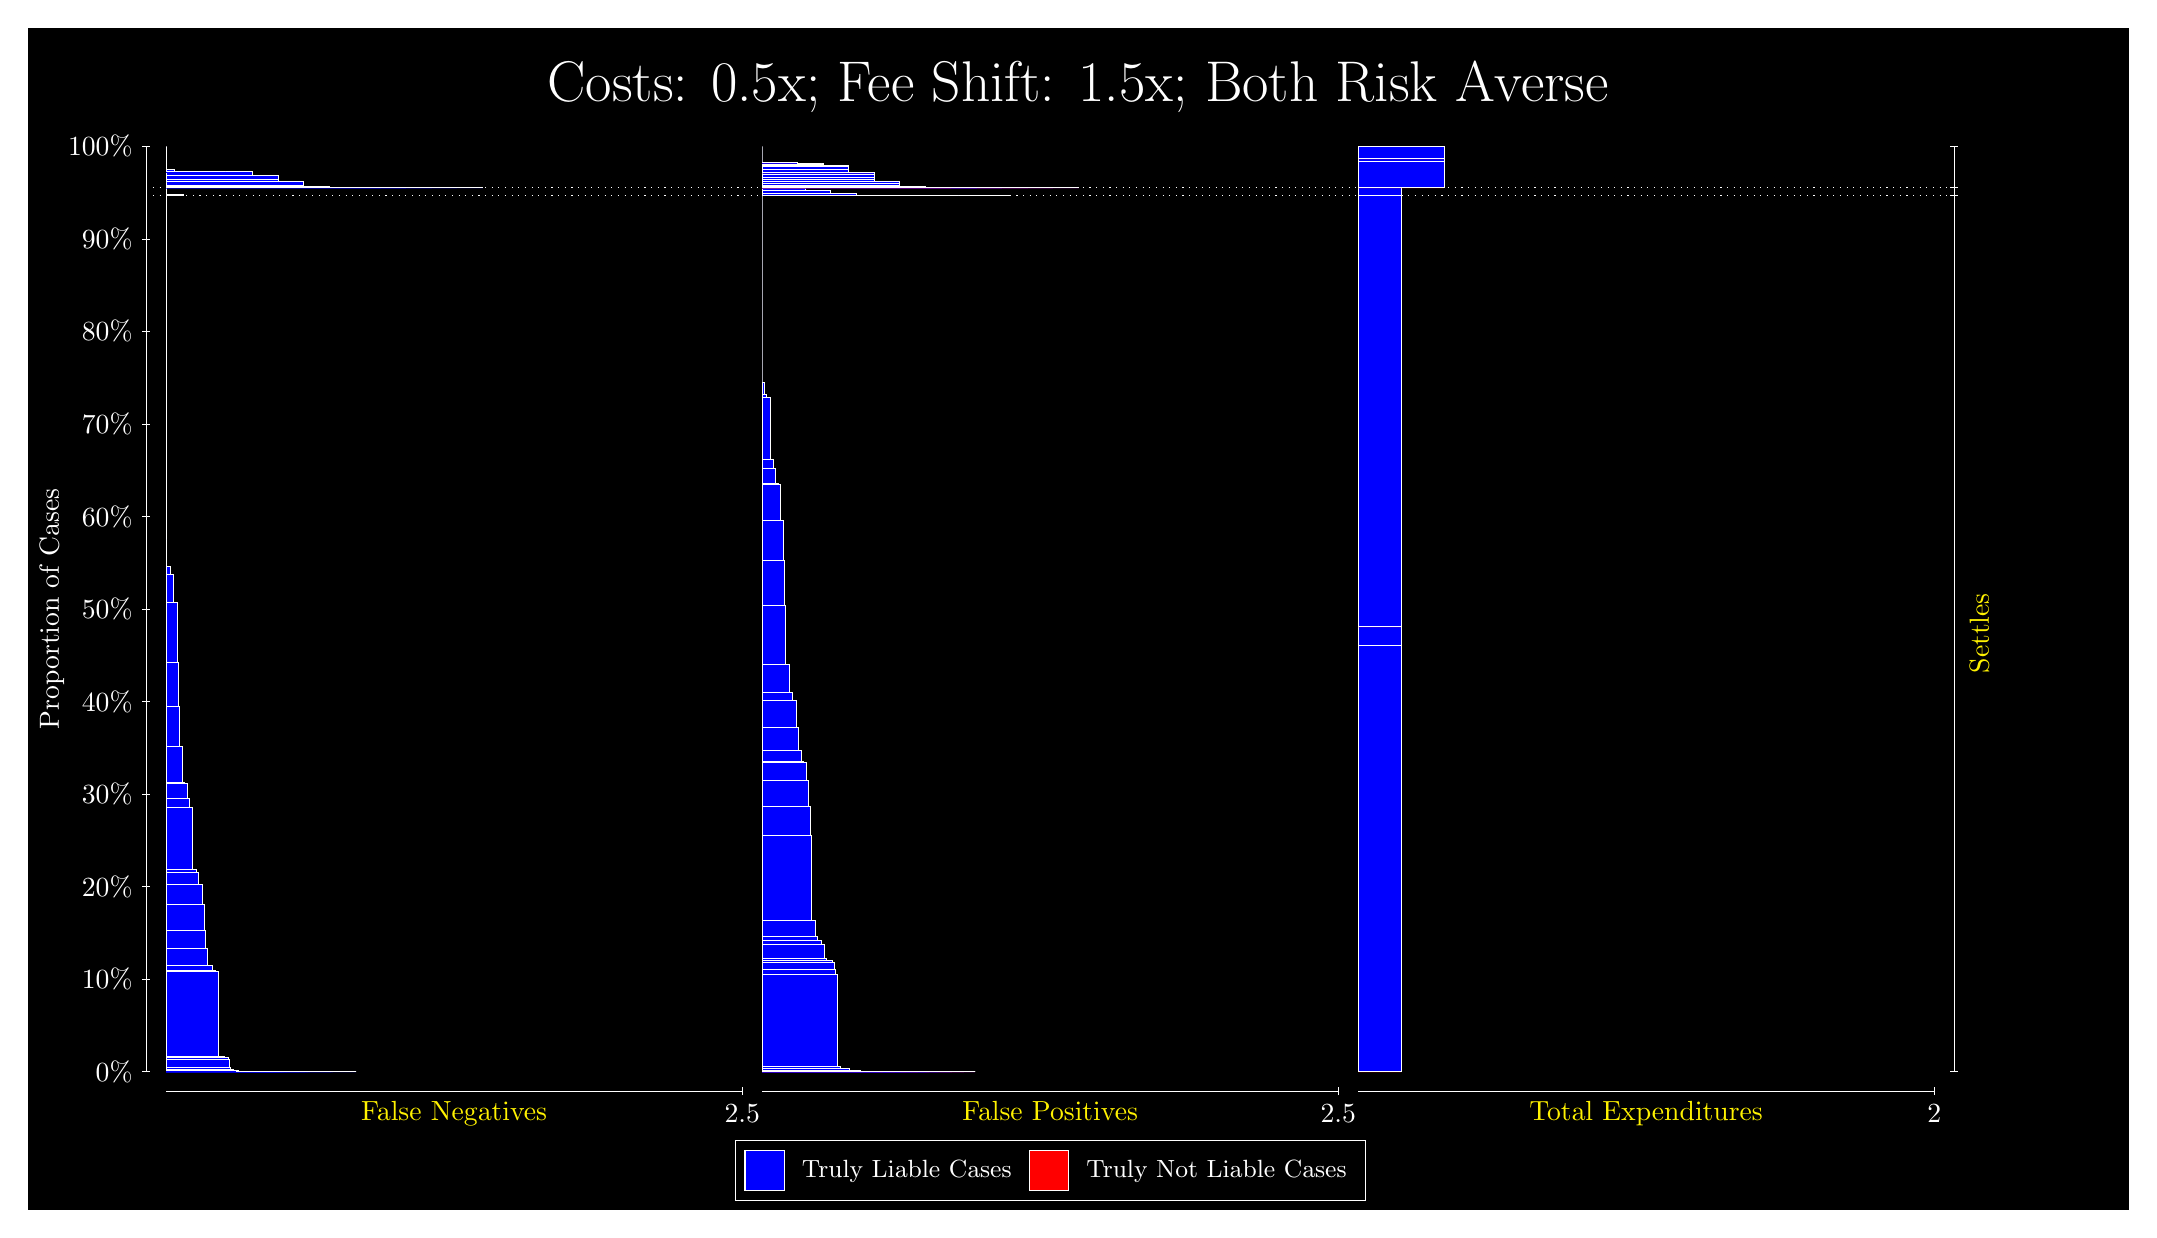
\begin{tikzpicture}
\draw[fill=black] (0,0) rectangle (26.667,15);
\draw[text=white] (0,13.5) rectangle (26.667,15) node[midway] {\huge Costs: 0.5x; Fee Shift: 1.5x; Both Risk Averse};
\draw[white, very thin] (1.5,1.75) -- (1.5,13.5);
\node[rotate=90, text=white, anchor=center] at (0.3, 7.625) {Proportion of Cases};
\draw[white, very thin] (1.45,1.75) -- (1.55,1.75);
\node[text=white, anchor=east] at (1.45, 1.75) {0\%};
\draw[white, very thin] (1.45,2.925) -- (1.55,2.925);
\node[text=white, anchor=east] at (1.45, 2.925) {10\%};
\draw[white, very thin] (1.45,4.1) -- (1.55,4.1);
\node[text=white, anchor=east] at (1.45, 4.1) {20\%};
\draw[white, very thin] (1.45,5.275) -- (1.55,5.275);
\node[text=white, anchor=east] at (1.45, 5.275) {30\%};
\draw[white, very thin] (1.45,6.45) -- (1.55,6.45);
\node[text=white, anchor=east] at (1.45, 6.45) {40\%};
\draw[white, very thin] (1.45,7.625) -- (1.55,7.625);
\node[text=white, anchor=east] at (1.45, 7.625) {50\%};
\draw[white, very thin] (1.45,8.8) -- (1.55,8.8);
\node[text=white, anchor=east] at (1.45, 8.8) {60\%};
\draw[white, very thin] (1.45,9.975) -- (1.55,9.975);
\node[text=white, anchor=east] at (1.45, 9.975) {70\%};
\draw[white, very thin] (1.45,11.15) -- (1.55,11.15);
\node[text=white, anchor=east] at (1.45, 11.15) {80\%};
\draw[white, very thin] (1.45,12.325) -- (1.55,12.325);
\node[text=white, anchor=east] at (1.45, 12.325) {90\%};
\draw[white, very thin] (1.45,13.5) -- (1.55,13.5);
\node[text=white, anchor=east] at (1.45, 13.5) {100\%};

\draw[white, very thin] (24.457,1.75) -- (24.457,13.5);
\draw[white, very thin] (24.407,1.75) -- (24.507,1.75);
\node[anchor=west] at (24.407, 1.75) {};
\draw[white, very thin] (24.407,12.881) -- (24.507,12.881);
\node[anchor=west] at (24.407, 12.881) {};
\draw[white, very thin] (24.407,12.976) -- (24.507,12.976);
\node[anchor=west] at (24.407, 12.976) {};
\draw[white, very thin] (24.407,13.5) -- (24.507,13.5);
\node[anchor=west] at (24.407, 13.5) {};

\draw[white, very thin, fill=blue] (1.75,1.75) rectangle (4.1652,1.75);
\draw[white, very thin, fill=blue] (1.75,1.75) rectangle (3.8725,1.75);
\draw[white, very thin, fill=blue] (1.75,1.75) rectangle (3.8399,1.75);
\draw[white, very thin, fill=blue] (1.75,1.75) rectangle (3.5797,1.75);
\draw[white, very thin, fill=blue] (1.75,1.75) rectangle (3.5472,1.75);
\draw[white, very thin, fill=blue] (1.75,1.75) rectangle (3.5147,1.75);
\draw[white, very thin, fill=blue] (1.75,1.75) rectangle (3.4333,1.75);
\draw[white, very thin, fill=blue] (1.75,1.75) rectangle (3.287,1.75);
\draw[white, very thin, fill=blue] (1.75,1.75) rectangle (3.2544,1.75);
\draw[white, very thin, fill=blue] (1.75,1.75) rectangle (3.2219,1.75);
\draw[white, very thin, fill=blue] (1.75,1.75) rectangle (3.1894,1.75);
\draw[white, very thin, fill=blue] (1.75,1.75) rectangle (3.1406,1.75);
\draw[white, very thin, fill=blue] (1.75,1.75) rectangle (3.1081,1.75);
\draw[white, very thin, fill=blue] (1.75,1.75) rectangle (2.9942,1.7504);
\draw[white, very thin, fill=blue] (1.75,1.7504) rectangle (2.9617,1.7504);
\draw[white, very thin, fill=blue] (1.75,1.7504) rectangle (2.9292,1.7509);
\draw[white, very thin, fill=blue] (1.75,1.7509) rectangle (2.8966,1.7514);
\draw[white, very thin, fill=blue] (1.75,1.7514) rectangle (2.8641,1.7519);
\draw[white, very thin, fill=blue] (1.75,1.7519) rectangle (2.8153,1.7521);
\draw[white, very thin, fill=blue] (1.75,1.7521) rectangle (2.7828,1.7522);
\draw[white, very thin, fill=blue] (1.75,1.7522) rectangle (2.7015,1.7526);
\draw[white, very thin, fill=blue] (1.75,1.7526) rectangle (2.6689,1.7601);
\draw[white, very thin, fill=blue] (1.75,1.7601) rectangle (2.6364,1.7604);
\draw[white, very thin, fill=blue] (1.75,1.7604) rectangle (2.6039,1.784);
\draw[white, very thin, fill=blue] (1.75,1.784) rectangle (2.5713,1.8078);
\draw[white, very thin, fill=blue] (1.75,1.8078) rectangle (2.5551,1.9077);
\draw[white, very thin, fill=blue] (1.75,1.9077) rectangle (2.5388,1.932);
\draw[white, very thin, fill=blue] (1.75,1.932) rectangle (2.49,1.9454);
\draw[white, very thin, fill=blue] (1.75,1.9454) rectangle (2.4575,1.9484);
\draw[white, very thin, fill=blue] (1.75,1.9484) rectangle (2.4087,3.0181);
\draw[white, very thin, fill=blue] (1.75,3.0181) rectangle (2.3762,3.0303);
\draw[white, very thin, fill=blue] (1.75,3.0303) rectangle (2.3436,3.0951);
\draw[white, very thin, fill=blue] (1.75,3.0951) rectangle (2.3111,3.0989);
\draw[white, very thin, fill=blue] (1.75,3.0989) rectangle (2.2786,3.3208);
\draw[white, very thin, fill=blue] (1.75,3.3208) rectangle (2.2461,3.5473);
\draw[white, very thin, fill=blue] (1.75,3.5473) rectangle (2.2298,3.878);
\draw[white, very thin, fill=blue] (1.75,3.878) rectangle (2.2135,4.1285);
\draw[white, very thin, fill=blue] (1.75,4.1285) rectangle (2.1647,4.2757);
\draw[white, very thin, fill=blue] (1.75,4.2757) rectangle (2.1322,4.3143);
\draw[white, very thin, fill=blue] (1.75,4.3143) rectangle (2.0834,5.1089);
\draw[white, very thin, fill=blue] (1.75,5.1089) rectangle (2.0509,5.2252);
\draw[white, very thin, fill=blue] (1.75,5.2252) rectangle (2.0184,5.4096);
\draw[white, very thin, fill=blue] (1.75,5.4096) rectangle (1.9858,5.4253);
\draw[white, very thin, fill=blue] (1.75,5.4253) rectangle (1.9533,5.8838);
\draw[white, very thin, fill=blue] (1.75,5.8838) rectangle (1.9208,6.3913);
\draw[white, very thin, fill=blue] (1.75,6.3913) rectangle (1.9045,6.9533);
\draw[white, very thin, fill=blue] (1.75,6.9533) rectangle (1.8882,7.7091);
\draw[white, very thin, fill=blue] (1.75,7.7091) rectangle (1.8395,8.0699);
\draw[white, very thin, fill=blue] (1.75,8.0699) rectangle (1.8069,8.1675);
\draw[white, very thin, fill=blue] (1.75,8.1675) rectangle (1.7581,8.5079);
\draw[white, very thin, fill=red] (1.75,8.5079) rectangle (1.75,8.5079);
\draw[white, very thin, fill=blue] (1.75,8.5079) rectangle (1.75,12.881);
\draw[white, very thin, fill=blue] (1.75,12.881) rectangle (1.9696,12.885);
\draw[white, very thin, fill=red] (1.75,12.885) rectangle (1.75,12.885);
\draw[white, very thin, fill=blue] (1.75,12.885) rectangle (1.75,12.976);
\draw[white, very thin, fill=blue] (1.75,12.976) rectangle (5.7754,12.976);
\draw[white, very thin, fill=blue] (1.75,12.976) rectangle (5.4501,12.976);
\draw[white, very thin, fill=blue] (1.75,12.976) rectangle (5.1248,12.976);
\draw[white, very thin, fill=blue] (1.75,12.976) rectangle (4.7995,12.976);
\draw[white, very thin, fill=blue] (1.75,12.976) rectangle (4.7995,12.976);
\draw[white, very thin, fill=blue] (1.75,12.976) rectangle (4.4742,12.976);
\draw[white, very thin, fill=blue] (1.75,12.976) rectangle (4.149,12.979);
\draw[white, very thin, fill=blue] (1.75,12.979) rectangle (3.8237,12.985);
\draw[white, very thin, fill=blue] (1.75,12.985) rectangle (3.8237,12.997);
\draw[white, very thin, fill=blue] (1.75,12.997) rectangle (3.4984,13.009);
\draw[white, very thin, fill=blue] (1.75,13.009) rectangle (3.4984,13.053);
\draw[white, very thin, fill=blue] (1.75,13.053) rectangle (3.4821,13.053);
\draw[white, very thin, fill=blue] (1.75,13.053) rectangle (3.1731,13.083);
\draw[white, very thin, fill=blue] (1.75,13.083) rectangle (3.1731,13.132);
\draw[white, very thin, fill=blue] (1.75,13.132) rectangle (3.1731,13.138);
\draw[white, very thin, fill=blue] (1.75,13.138) rectangle (3.1568,13.138);
\draw[white, very thin, fill=blue] (1.75,13.138) rectangle (3.1568,13.138);
\draw[white, very thin, fill=blue] (1.75,13.138) rectangle (2.8478,13.178);
\draw[white, very thin, fill=blue] (1.75,13.178) rectangle (2.8316,13.178);
\draw[white, very thin, fill=blue] (1.75,13.178) rectangle (2.5225,13.18);
\draw[white, very thin, fill=blue] (1.75,13.18) rectangle (2.5225,13.182);
\draw[white, very thin, fill=blue] (1.75,13.182) rectangle (2.5225,13.183);
\draw[white, very thin, fill=blue] (1.75,13.183) rectangle (2.5063,13.183);
\draw[white, very thin, fill=blue] (1.75,13.183) rectangle (2.5063,13.183);
\draw[white, very thin, fill=blue] (1.75,13.183) rectangle (2.1973,13.183);
\draw[white, very thin, fill=blue] (1.75,13.183) rectangle (2.1973,13.183);
\draw[white, very thin, fill=blue] (1.75,13.183) rectangle (2.181,13.184);
\draw[white, very thin, fill=blue] (1.75,13.184) rectangle (1.872,13.184);
\draw[white, very thin, fill=blue] (1.75,13.184) rectangle (1.872,13.184);
\draw[white, very thin, fill=blue] (1.75,13.184) rectangle (1.8557,13.187);
\draw[white, very thin, fill=blue] (1.75,13.187) rectangle (1.8557,13.212);
\draw[white, very thin, fill=red] (1.75,13.212) rectangle (1.75,13.212);
\draw[white, very thin, fill=blue] (1.75,13.212) rectangle (1.75,13.5);
\draw[white, very thin, fill=red] (9.3189,1.75) rectangle (12.027,1.75);
\draw[white, very thin, fill=blue] (9.3189,1.75) rectangle (12.027,1.75);
\draw[white, very thin, fill=red] (9.3189,1.75) rectangle (11.88,1.75);
\draw[white, very thin, fill=blue] (9.3189,1.75) rectangle (11.88,1.75);
\draw[white, very thin, fill=red] (9.3189,1.75) rectangle (11.734,1.75);
\draw[white, very thin, fill=blue] (9.3189,1.75) rectangle (11.734,1.75);
\draw[white, very thin, fill=blue] (9.3189,1.75) rectangle (11.702,1.75);
\draw[white, very thin, fill=blue] (9.3189,1.75) rectangle (11.555,1.75);
\draw[white, very thin, fill=red] (9.3189,1.75) rectangle (11.441,1.75);
\draw[white, very thin, fill=blue] (9.3189,1.75) rectangle (11.441,1.75);
\draw[white, very thin, fill=blue] (9.3189,1.75) rectangle (11.409,1.75);
\draw[white, very thin, fill=blue] (9.3189,1.75) rectangle (11.376,1.75);
\draw[white, very thin, fill=red] (9.3189,1.75) rectangle (11.295,1.75);
\draw[white, very thin, fill=blue] (9.3189,1.75) rectangle (11.295,1.75);
\draw[white, very thin, fill=blue] (9.3189,1.75) rectangle (11.23,1.75);
\draw[white, very thin, fill=red] (9.3189,1.75) rectangle (11.149,1.75);
\draw[white, very thin, fill=blue] (9.3189,1.75) rectangle (11.149,1.75);
\draw[white, very thin, fill=blue] (9.3189,1.75) rectangle (11.116,1.75);
\draw[white, very thin, fill=blue] (9.3189,1.75) rectangle (11.084,1.75);
\draw[white, very thin, fill=blue] (9.3189,1.75) rectangle (11.051,1.75);
\draw[white, very thin, fill=red] (9.3189,1.75) rectangle (11.002,1.75);
\draw[white, very thin, fill=blue] (9.3189,1.75) rectangle (11.002,1.75);
\draw[white, very thin, fill=blue] (9.3189,1.75) rectangle (10.97,1.75);
\draw[white, very thin, fill=blue] (9.3189,1.75) rectangle (10.905,1.75);
\draw[white, very thin, fill=red] (9.3189,1.75) rectangle (10.856,1.75);
\draw[white, very thin, fill=blue] (9.3189,1.75) rectangle (10.856,1.75);
\draw[white, very thin, fill=blue] (9.3189,1.75) rectangle (10.823,1.75);
\draw[white, very thin, fill=blue] (9.3189,1.75) rectangle (10.791,1.7501);
\draw[white, very thin, fill=blue] (9.3189,1.7501) rectangle (10.758,1.7505);
\draw[white, very thin, fill=blue] (9.3189,1.7505) rectangle (10.726,1.7506);
\draw[white, very thin, fill=blue] (9.3189,1.7506) rectangle (10.677,1.7508);
\draw[white, very thin, fill=blue] (9.3189,1.7508) rectangle (10.644,1.7513);
\draw[white, very thin, fill=blue] (9.3189,1.7513) rectangle (10.579,1.7544);
\draw[white, very thin, fill=red] (9.3189,1.7544) rectangle (10.563,1.7544);
\draw[white, very thin, fill=blue] (9.3189,1.7544) rectangle (10.563,1.7649);
\draw[white, very thin, fill=blue] (9.3189,1.7649) rectangle (10.531,1.7655);
\draw[white, very thin, fill=blue] (9.3189,1.7655) rectangle (10.498,1.7656);
\draw[white, very thin, fill=blue] (9.3189,1.7656) rectangle (10.465,1.7669);
\draw[white, very thin, fill=blue] (9.3189,1.7669) rectangle (10.433,1.7877);
\draw[white, very thin, fill=blue] (9.3189,1.7877) rectangle (10.4,1.7909);
\draw[white, very thin, fill=blue] (9.3189,1.7909) rectangle (10.352,1.7976);
\draw[white, very thin, fill=blue] (9.3189,1.7976) rectangle (10.319,1.8201);
\draw[white, very thin, fill=red] (9.3189,1.8201) rectangle (10.27,1.8201);
\draw[white, very thin, fill=blue] (9.3189,1.8201) rectangle (10.27,2.9842);
\draw[white, very thin, fill=blue] (9.3189,2.9842) rectangle (10.254,3.0534);
\draw[white, very thin, fill=blue] (9.3189,3.0534) rectangle (10.238,3.1366);
\draw[white, very thin, fill=blue] (9.3189,3.1366) rectangle (10.205,3.1606);
\draw[white, very thin, fill=blue] (9.3189,3.1606) rectangle (10.173,3.1634);
\draw[white, very thin, fill=blue] (9.3189,3.1634) rectangle (10.14,3.1924);
\draw[white, very thin, fill=blue] (9.3189,3.1924) rectangle (10.108,3.3628);
\draw[white, very thin, fill=blue] (9.3189,3.3628) rectangle (10.075,3.4216);
\draw[white, very thin, fill=blue] (9.3189,3.4216) rectangle (10.026,3.4731);
\draw[white, very thin, fill=blue] (9.3189,3.4731) rectangle (9.9938,3.6705);
\draw[white, very thin, fill=blue] (9.3189,3.6705) rectangle (9.945,4.7541);
\draw[white, very thin, fill=blue] (9.3189,4.7541) rectangle (9.9288,5.1169);
\draw[white, very thin, fill=blue] (9.3189,5.1169) rectangle (9.9125,5.4504);
\draw[white, very thin, fill=blue] (9.3189,5.4504) rectangle (9.88,5.6723);
\draw[white, very thin, fill=blue] (9.3189,5.6723) rectangle (9.8475,5.6867);
\draw[white, very thin, fill=blue] (9.3189,5.6867) rectangle (9.8149,5.8333);
\draw[white, very thin, fill=blue] (9.3189,5.8333) rectangle (9.7824,6.1228);
\draw[white, very thin, fill=blue] (9.3189,6.1228) rectangle (9.7499,6.4632);
\draw[white, very thin, fill=blue] (9.3189,6.4632) rectangle (9.7011,6.5607);
\draw[white, very thin, fill=blue] (9.3189,6.5607) rectangle (9.6685,6.9216);
\draw[white, very thin, fill=blue] (9.3189,6.9216) rectangle (9.6198,7.6773);
\draw[white, very thin, fill=blue] (9.3189,7.6773) rectangle (9.6035,8.2393);
\draw[white, very thin, fill=blue] (9.3189,8.2393) rectangle (9.5872,8.7469);
\draw[white, very thin, fill=blue] (9.3189,8.7469) rectangle (9.5547,9.2054);
\draw[white, very thin, fill=blue] (9.3189,9.2054) rectangle (9.5222,9.2211);
\draw[white, very thin, fill=blue] (9.3189,9.2211) rectangle (9.4896,9.4055);
\draw[white, very thin, fill=blue] (9.3189,9.4055) rectangle (9.4571,9.5218);
\draw[white, very thin, fill=blue] (9.3189,9.5218) rectangle (9.4246,10.316);
\draw[white, very thin, fill=blue] (9.3189,10.316) rectangle (9.3758,10.355);
\draw[white, very thin, fill=blue] (9.3189,10.355) rectangle (9.3433,10.502);
\draw[white, very thin, fill=blue] (9.3189,10.502) rectangle (9.3189,12.881);
\draw[white, very thin, fill=red] (9.3189,12.881) rectangle (12.466,12.881);
\draw[white, very thin, fill=blue] (9.3189,12.881) rectangle (12.466,12.881);
\draw[white, very thin, fill=blue] (9.3189,12.881) rectangle (12.141,12.881);
\draw[white, very thin, fill=blue] (9.3189,12.881) rectangle (11.815,12.881);
\draw[white, very thin, fill=blue] (9.3189,12.881) rectangle (11.49,12.881);
\draw[white, very thin, fill=blue] (9.3189,12.881) rectangle (11.165,12.881);
\draw[white, very thin, fill=blue] (9.3189,12.881) rectangle (10.84,12.882);
\draw[white, very thin, fill=blue] (9.3189,12.882) rectangle (10.514,12.902);
\draw[white, very thin, fill=blue] (9.3189,12.902) rectangle (10.189,12.947);
\draw[white, very thin, fill=blue] (9.3189,12.947) rectangle (9.8637,12.971);
\draw[white, very thin, fill=blue] (9.3189,12.971) rectangle (9.5384,12.976);
\draw[white, very thin, fill=red] (9.3189,12.976) rectangle (13.344,12.976);
\draw[white, very thin, fill=blue] (9.3189,12.976) rectangle (13.344,12.976);
\draw[white, very thin, fill=red] (9.3189,12.976) rectangle (13.019,12.976);
\draw[white, very thin, fill=blue] (9.3189,12.976) rectangle (13.019,12.976);
\draw[white, very thin, fill=red] (9.3189,12.976) rectangle (12.694,12.976);
\draw[white, very thin, fill=blue] (9.3189,12.976) rectangle (12.694,12.976);
\draw[white, very thin, fill=blue] (9.3189,12.976) rectangle (12.368,12.976);
\draw[white, very thin, fill=red] (9.3189,12.976) rectangle (12.368,12.976);
\draw[white, very thin, fill=blue] (9.3189,12.976) rectangle (12.368,12.976);
\draw[white, very thin, fill=red] (9.3189,12.976) rectangle (12.043,12.976);
\draw[white, very thin, fill=blue] (9.3189,12.976) rectangle (12.043,12.976);
\draw[white, very thin, fill=blue] (9.3189,12.976) rectangle (12.043,12.976);
\draw[white, very thin, fill=blue] (9.3189,12.976) rectangle (12.043,12.976);
\draw[white, very thin, fill=red] (9.3189,12.976) rectangle (11.718,12.976);
\draw[white, very thin, fill=blue] (9.3189,12.976) rectangle (11.718,12.979);
\draw[white, very thin, fill=blue] (9.3189,12.979) rectangle (11.718,12.979);
\draw[white, very thin, fill=blue] (9.3189,12.979) rectangle (11.393,12.985);
\draw[white, very thin, fill=red] (9.3189,12.985) rectangle (11.393,12.985);
\draw[white, very thin, fill=blue] (9.3189,12.985) rectangle (11.393,12.998);
\draw[white, very thin, fill=blue] (9.3189,12.998) rectangle (11.067,13.011);
\draw[white, very thin, fill=blue] (9.3189,13.011) rectangle (11.067,13.03);
\draw[white, very thin, fill=blue] (9.3189,13.03) rectangle (11.067,13.056);
\draw[white, very thin, fill=red] (9.3189,13.056) rectangle (11.051,13.056);
\draw[white, very thin, fill=blue] (9.3189,13.056) rectangle (11.051,13.056);
\draw[white, very thin, fill=blue] (9.3189,13.056) rectangle (10.742,13.08);
\draw[white, very thin, fill=blue] (9.3189,13.08) rectangle (10.742,13.103);
\draw[white, very thin, fill=blue] (9.3189,13.103) rectangle (10.742,13.14);
\draw[white, very thin, fill=blue] (9.3189,13.14) rectangle (10.742,13.165);
\draw[white, very thin, fill=red] (9.3189,13.165) rectangle (10.726,13.165);
\draw[white, very thin, fill=blue] (9.3189,13.165) rectangle (10.726,13.165);
\draw[white, very thin, fill=blue] (9.3189,13.165) rectangle (10.726,13.165);
\draw[white, very thin, fill=blue] (9.3189,13.165) rectangle (10.417,13.211);
\draw[white, very thin, fill=blue] (9.3189,13.211) rectangle (10.417,13.241);
\draw[white, very thin, fill=blue] (9.3189,13.241) rectangle (10.417,13.264);
\draw[white, very thin, fill=blue] (9.3189,13.264) rectangle (10.4,13.264);
\draw[white, very thin, fill=red] (9.3189,13.264) rectangle (10.4,13.264);
\draw[white, very thin, fill=blue] (9.3189,13.264) rectangle (10.4,13.264);
\draw[white, very thin, fill=blue] (9.3189,13.264) rectangle (10.091,13.275);
\draw[white, very thin, fill=blue] (9.3189,13.275) rectangle (10.091,13.29);
\draw[white, very thin, fill=blue] (9.3189,13.29) rectangle (10.091,13.291);
\draw[white, very thin, fill=blue] (9.3189,13.291) rectangle (10.075,13.291);
\draw[white, very thin, fill=blue] (9.3189,13.291) rectangle (10.075,13.291);
\draw[white, very thin, fill=red] (9.3189,13.291) rectangle (10.075,13.291);
\draw[white, very thin, fill=blue] (9.3189,13.291) rectangle (10.075,13.291);
\draw[white, very thin, fill=blue] (9.3189,13.291) rectangle (9.7661,13.292);
\draw[white, very thin, fill=blue] (9.3189,13.292) rectangle (9.7661,13.293);
\draw[white, very thin, fill=blue] (9.3189,13.293) rectangle (9.7499,13.293);
\draw[white, very thin, fill=blue] (9.3189,13.293) rectangle (9.7499,13.293);
\draw[white, very thin, fill=red] (9.3189,13.293) rectangle (9.7499,13.293);
\draw[white, very thin, fill=blue] (9.3189,13.293) rectangle (9.7499,13.293);
\draw[white, very thin, fill=blue] (9.3189,13.293) rectangle (9.7499,13.293);
\draw[white, very thin, fill=blue] (9.3189,13.293) rectangle (9.4408,13.293);
\draw[white, very thin, fill=blue] (9.3189,13.293) rectangle (9.4408,13.293);
\draw[white, very thin, fill=blue] (9.3189,13.293) rectangle (9.4408,13.293);
\draw[white, very thin, fill=blue] (9.3189,13.293) rectangle (9.4246,13.293);
\draw[white, very thin, fill=blue] (9.3189,13.293) rectangle (9.4246,13.294);
\draw[white, very thin, fill=red] (9.3189,13.294) rectangle (9.4246,13.294);
\draw[white, very thin, fill=blue] (9.3189,13.294) rectangle (9.4246,13.296);
\draw[white, very thin, fill=blue] (9.3189,13.296) rectangle (9.4246,13.297);
\draw[white, very thin, fill=red] (9.3189,13.297) rectangle (9.3189,13.297);
\draw[white, very thin, fill=blue] (9.3189,13.297) rectangle (9.3189,13.5);
\draw[white, very thin, fill=red] (16.888,1.75) rectangle (17.437,1.75);
\draw[white, very thin, fill=blue] (16.888,1.75) rectangle (17.437,7.1652);
\draw[white, very thin, fill=red] (16.888,7.1652) rectangle (17.437,7.1652);
\draw[white, very thin, fill=blue] (16.888,7.1652) rectangle (17.437,7.3998);
\draw[white, very thin, fill=red] (16.888,7.3998) rectangle (17.437,7.3998);
\draw[white, very thin, fill=blue] (16.888,7.3998) rectangle (17.437,12.881);
\draw[white, very thin, fill=red] (16.888,12.881) rectangle (17.437,12.881);
\draw[white, very thin, fill=blue] (16.888,12.881) rectangle (17.437,12.976);
\draw[white, very thin, fill=red] (16.888,12.976) rectangle (17.986,12.976);
\draw[white, very thin, fill=blue] (16.888,12.976) rectangle (17.986,13.314);
\draw[white, very thin, fill=red] (16.888,13.314) rectangle (17.986,13.314);
\draw[white, very thin, fill=blue] (16.888,13.314) rectangle (17.986,13.342);
\draw[white, very thin, fill=red] (16.888,13.342) rectangle (17.986,13.342);
\draw[white, very thin, fill=blue] (16.888,13.342) rectangle (17.986,13.5);
\draw[white, dotted] (1.5,12.881) -- (24.457,12.881);
\draw[white, dotted] (1.5,12.976) -- (24.457,12.976);
\draw[white, very thin] (1.75,1.5) -- (9.0689,1.5);
\node[text=yellow, anchor=north] at (5.4094, 1.5) {False Negatives};
\draw[white, very thin] (9.0689,1.45) -- (9.0689,1.55);
\node[text=white, anchor=north] at (9.0689, 1.45) {2.5};

\draw[white, very thin] (9.3189,1.5) -- (16.638,1.5);
\node[text=yellow, anchor=north] at (12.978, 1.5) {False Positives};
\draw[white, very thin] (16.638,1.45) -- (16.638,1.55);
\node[text=white, anchor=north] at (16.638, 1.45) {2.5};

\draw[white, very thin] (16.888,1.5) -- (24.207,1.5);
\node[text=yellow, anchor=north] at (20.547, 1.5) {Total Expenditures};
\draw[white, very thin] (24.207,1.45) -- (24.207,1.55);
\node[text=white, anchor=north] at (24.207, 1.45) {2};

\node[text=yellow, centered, rotate=90] at (24.777, 7.3153) {Settles};



\draw (12.978300999999998,1.5) node[draw=none] (baseCoordinate) {};
\begin{scope}[align=center]
        \matrix[scale=0.5, draw=white, below=0.5cm of baseCoordinate, nodes={draw}, column sep=0.1cm]{
            \node[rectangle, draw, minimum width=0.5cm, minimum height=0.5cm, fill=blue] {}; &
            \node[draw=none, font=\small, text=white] (B) {Truly Liable Cases}; &
            \node[rectangle, draw, minimum width=0.5cm, minimum height=0.5cm, fill=red] {}; &
            \node[draw=none, font=\small, text=white] (B) {Truly Not Liable Cases}; \\
            };
\end{scope}

\end{tikzpicture}
\end{document}